\section{AC CIRCUIT}
\subsection{AC-01}
\begin{figure}[h]
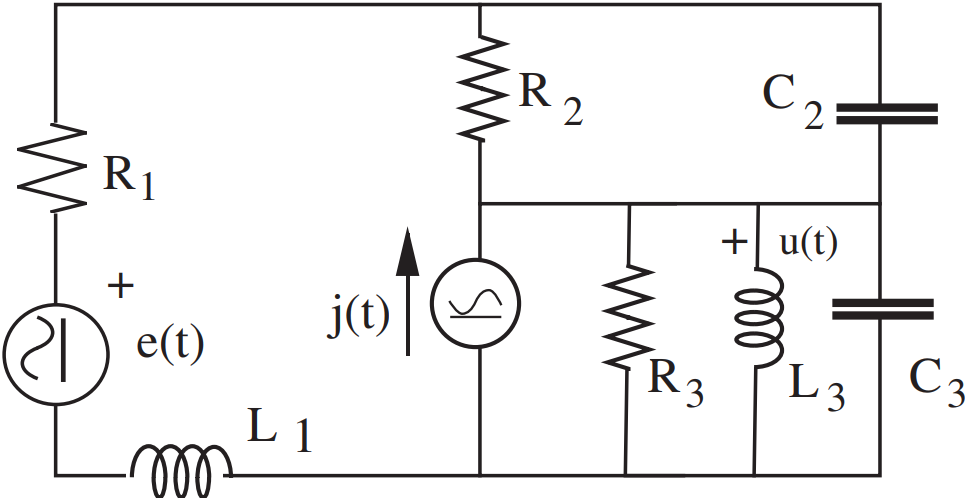
\includegraphics[height=6cm]{img/2/01.png}
\centering
\end{figure}
\begin{center}
\begin{tabular}{ c c c }
  $j(t) = 30\ \sin{(100t + \dfrac{\pi}{4})}$ & $e(t) =300 \sqrt{2} \ \sin{(100t + \dfrac{\pi}{2})}$ & $R_1 = R_3 = 10 \ \Omega$\\
  $R_2 = 20 \ \Omega$ & $L_1 = 400\ mH $ & $L_3 = 400\ mH $\\
  $C_2 = 500 \ \mu F$ & $C_3 = 250 \ \mu F$\\
\end{tabular}
\end{center}
\textbf{Determine}:
\begin{itemize}
  \item $u(t)$
  \item $P\ped{j}$ and $Q\ped{j}$
  \item $P\ped{e}$ and $Q\ped{e}$
\end{itemize}
\underline{\large{Solution:}}
\newline
$u(t) =250 \sqrt{2} \ \sin{(100t + 0.9273)}$, $P\ped{j} = 5250\ W$, $Q\ped{j} = 750\ var$, $P\ped{e} = 1500\ W$\\
$Q\ped{e} = 3.3448\ \cdot 10^{-13}\ var$
\subsection{AC-02}
\begin{figure}[h]
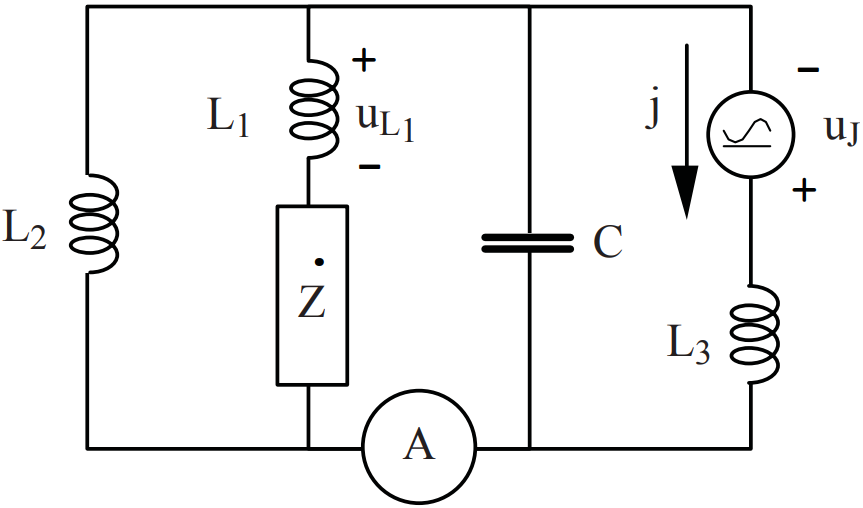
\includegraphics[height=6cm]{img/2/02.png}
\centering
\end{figure}
\begin{center}
\begin{tabular}{ c c c c }
    $L_1 = 10\ mH $ & $L_2 = 15\ mH $ & $L_3 = 15\ mH $ & $C = 25\ \mu F$\\ $u\ped{L_1}(t) = 320\ \cdot\ \sin{(1000t + \dfrac{\pi}{4})}$ & $I_A = 0\ A$
\end{tabular}
\end{center}
\textbf{Determine}:
\begin{itemize}
  \item $\Dot{Z} = R + j X$
  \item $Q\ped{L_2}$
  \item $j(t)$ and  $u\ped{j}(t)$ 
  \item $Q\ped{L_3}$
\end{itemize}
\underline{\large{Solution:}}
\newline
$\Dot{Z} = -25i$, $Q\ped{L_2} = 7680\ var$, $j(t) = 12\ \cdot\ \sin{(1000t + \dfrac{3}{4}\ \pi )}$, $u\ped{j}(t) = 300\ \cdot\ \sin{(1000t + \dfrac{\pi}{4}\ )}$, $Q\ped{L_3} = 1080\ var$
\subsection{AC-03}
\begin{figure}[h]
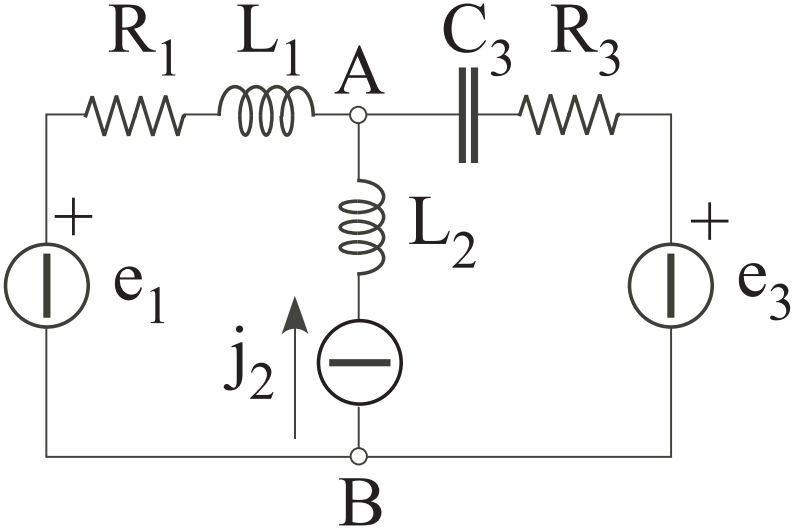
\includegraphics[height=6cm]{img/2/03.png}
\centering
\end{figure}
\begin{center}
\begin{tabular}{ c c c }
    $e\ped{1}(t) = 100\ \sin{(1000t)}$ & $j\ped{2}(t) = 8\ \cos{(1000t)}$ & $e\ped{3}(t) = 200\ \sin{(1000t)}$\\
    $R_1 = 5\ \Omega$ & $R_3 = 10\ \Omega$ & $L_1 = 5\ mH$ \\
    $L_2 = 10\ mH$ & $C_3 = 100\ \mu F$
\end{tabular}
\end{center}
\textbf{Determine}:
\begin{itemize}
  \item $P\ped{R_1}$ and $P\ped{R_3}$
  \item $P\ped{E_1}$, $P\ped{J_2}$ and $P\ped{E_3}$ 
  \item $S\ped{J_2}$ 
  \item $i\ped{e_3}(t)$
\end{itemize}
\underline{\large{Solution:}}
\newline
$P\ped{R_1} = 776\ W$, $P\ped{R_3} = 848\ W$, $P\ped{E_1} = -920\ W$, $P\ped{J_2} = 704\ W$, $P\ped{E_3} = 1840\ W$, $S\ped{J_2} = 729.71\ $VA, $i\ped{e_3}(t) = 13.023\ \sin{(1000t + 0.043451 )}$
\newpage
\subsection{AC-04}
\begin{figure}[h]
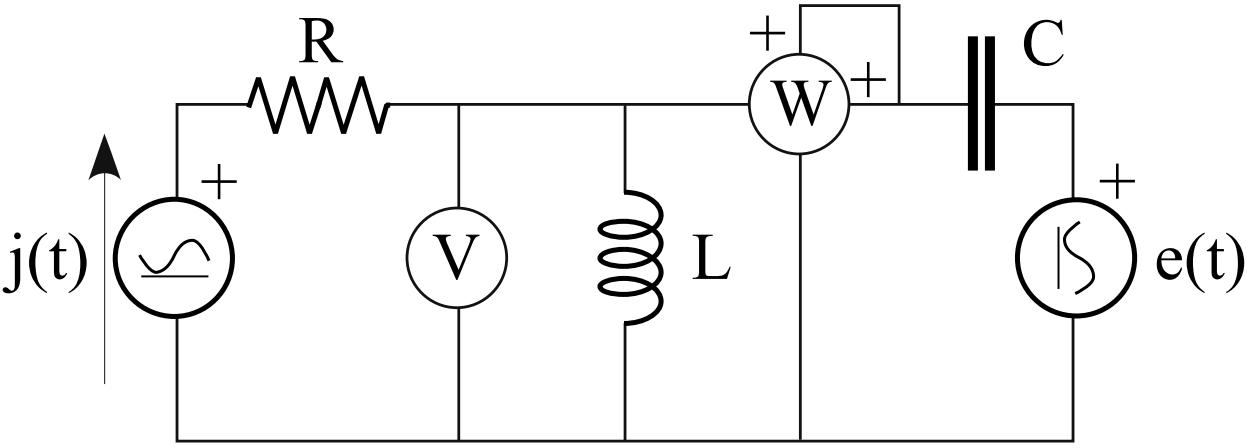
\includegraphics[height=5cm]{img/2/04.png}
\centering
\end{figure}
\begin{center}
\begin{tabular}{ c c c }
    $e(t) = 100 \cdot \sqrt{2}\ \sin{(200t)}$ & $j(t) = 10 \cdot \sqrt{2} \sin{(200t + \pi)}$ & $R = 5\ \Omega$\\
    $L = 100\ mH$ & $C = 500\ \mu F$\\
\end{tabular}
\end{center}
\textbf{Determine}:
\begin{itemize}
  \item The indication of the voltmeter $U_V$
  \item $P\ped{W}$ 
  \item $u\ped{j}(t)$
  \item $i\ped{e}(t)$
  \item $P\ped{j}$ and $Q\ped{j}$
\end{itemize}
\underline{\large{Solution:}}
\newline
$U_V = 282.84\ V$, $P\ped{W} = 2000\ W$, $u\ped{j}(t) = 353.55\ \cdot\ \sin{(200t + 0.9273 )}$, $i\ped{e}(t) = 31.623\ \cdot\ \sin{(200t - 0.46365 )}$\\
$P\ped{j} = -1500\ W$,  $Q\ped{j} = -2000\ var$
\newline